\begin{tikzpicture}[thick, scale=0.7, every node/.style={transform shape}]
    % Axes
    \def\x{6}\def\y{3.5}
    \draw[-] (-0.5,0) -- (\x+0.5,0) node[right] {};
    \draw[-] (0,-0.5) -- (0,\y+0.5);

    \node (A) at (1.5, 3) {};
    \node (B) at (3.5, 1) {};
    \node (C) at ($(A)!0.5!(B)$) {};
    \draw[{|-|}, very thick] (A) -- (B);

    \fill [red!80] (A) circle (2pt) node[above, black] {$\mu_{P}$};
    \fill [red!80] (B) circle (2pt) node[below, black] {$\mu_{Q}$};
    \node (MMD) at (4.5, 3.5) {$\left\lVert \mu_{P} - \mu_{Q}\right\lVert_{\iH(k)}$};
    \draw[-stealth] (MMD) to [bend left] (C);

    \node [inner sep=0pt] (disc) at (-2,0.9) {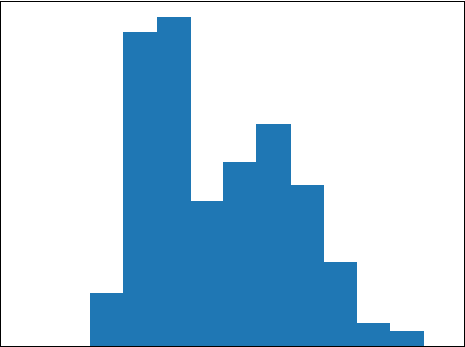
\includegraphics[width=.2\textwidth]{part2/figures/WAKE/discrete.pdf}};
    \node [inner sep=0pt] (cont) at (-2,3.1) {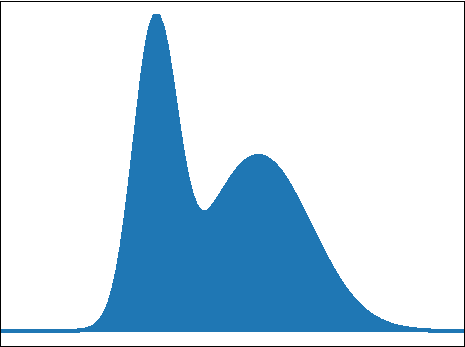
\includegraphics[width=.2\textwidth]{part2/figures/WAKE/continuous.pdf}};
    \draw[-stealth] (cont) to [bend left] (A);
    \draw[-stealth] (disc.east) to [bend right] (B);
    % Text
    \node at (5, 0.25) {$\mathcal{H}_k$};
    \node at (-3, 3) {$P$};
    \node at (-3, 1) {$Q$};
\end{tikzpicture}